\question{Многоэлектронные атомы. Векторная модель многоэлектронного 
атома. Магнитный момент многоэлектронного атома. Фактор Ланде.}

Механический и магнитный моменты связаны гиромагнитным отношением, но в случае
спиновых моментов, это отношение в два раза больше:
\[
    \mu_L = -\mu_\emph{Б}\sqrt{L(L+1)}, \quad \mu_S = -2\mu_\emph{Б}
    \sqrt{S(S+1)}, \quad \mu_J = -\mu_\emph{Б}g\sqrt{J(J+1)},
\]
где
\[
    g = 1 + \frac{J(J+1) + S(S+1) - L(L+1)}{2J(J+1)} \text{ -- фактор Ланде}.
\]

\subquestion{Векторная модель многоэлектронного атома}

Из-за удвоенного магнетизма спина, \( \mu_J \) начинает прецессировать вокруг
оси, совпадающей с осью, проходящей через \( \vec{M}_J \):

\begin{gather*}
    \average{\mu_{J_z}} = -|\mu_L|\cos\alpha - |\mu_S|\cos\beta; \\
    |\mu_L| = \mu_\emph{Б}\sqrt{L(L+1)}, \quad |\mu_S| = 2\mu_\emph{Б}
    \sqrt{S(S+1)};\\
    M_S^2 = M_L^2 + M_J^2 - 2M_L M_J\cos\alpha, \quad \cos\alpha =
    \frac{-M_S^2 + M_L^2 + M_J^2}{2M_L M_J} = \frac{L(L+1) + J(J+1) - S(S+1)}
    {2\sqrt{L(L+1)}\sqrt{J(J+1)}}; \\
    M_L^2 = M_J^2 + M_S^2 - 2M_J M_S\cos\beta, \quad \cos\beta =
    \frac{M_J^2 + M_S^2 - M_L^2}{2M_S M_J} = \frac{J(J+1) + S(S+1) - L(L+1)}
    {2\sqrt{J(J+1)}\sqrt{S(S+1)}}; \\
    \average{\mu_{J_z}} = -\mu_\emph{Б}\frac{L(L+1) + J(J+1) - S(S+1)}
    {2\sqrt{J(J+1)}} - 2\mu_\emph{Б}\frac{J(J+1) + S(S+1) - L(L+1)}
    {2\sqrt{J(J+1)}}; \\
    \average{\mu_{J_z}} = - \mu_\emph{Б}\frac{3J(J+1) + S(S+1) - L(L+1)}
    {2\sqrt{J(J+1)}} = -\mu_\emph{Б}g\sqrt{J(J+1)} = \mu_J.
\end{gather*}

\begin{figure}[h!]
    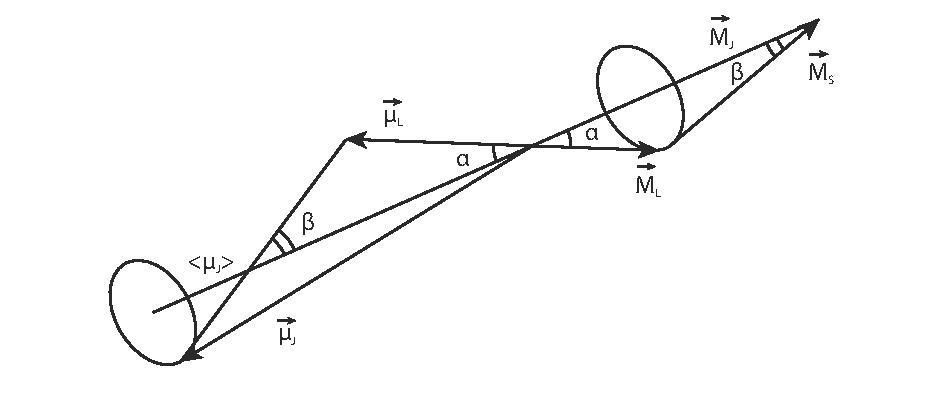
\includegraphics[width=.5\textwidth]{11_01}
\end{figure}

\newpage
